\section{Overview}
In the setting of sidechains, we wish to transfer assets from one blockchain to
another and then back. When assets can be transferred from one blockchain to
another but not back, we call it a \emph{one-way peg}. If assets can also be
moved back, we call it a \emph{two-way peg}. In each individual transfer of an
asset, we have a particular \emph{source blockchain}, from which the asset is
moved, and a particular \emph{target blockchain}, to which the asset is moved.
In a sidechain setting of two blockchains that are two-way pegged, both
blockchains can function as a source and a target blockchain for different
transfers.

While the motivation for the construction is to be able to move assets from one
blockchain to another, we wish to generalize the notion of sidechains from this
strict setting. In general, we would like the target blockchain to be able to
react to any \emph{event} that can occur on the source blockchain. Events within
a blockchain are any conditions to which local (to the particular blockchain)
smart contracts can react. For example, such events can be the fact that a
transaction with a particular \textsc{txid} took place, that a certain account
was paid a certain amount of money, or that a particular smart contract was
instantiated. Our sidechain construction allows the target blockchain to react
to events that took place on source blockchain in its target blockchain smart
contracts. We will describe our construction in pseudocode which is similar to
Ethereum' \emph{Solidity} and can be readily implemented there from our
high-level description. In this setting, events are defined by Solidity using
the \textsf{event} type and have an \emph{event name}, a \emph{contract address}
which fired them, as well as certain parameter values.

\begin{figure}
    \caption{The source blockchain, pictured at the top, fires an event
             included in the black block. The event is confirmed by being buried
             under $k_1$ blocks in the source blockchain. The target blockchain,
             pictured at the bottom, reacts to the event with an action included
             in the white block. The white block is subsequently confirmed by
             being buried under $k_2$ blocks. Arrows between blocks of the same
             blockchain indicate authenticated ancestry. The arrow between the
             two blockchains indicates the data transfer needed for the event.}
    \centering
    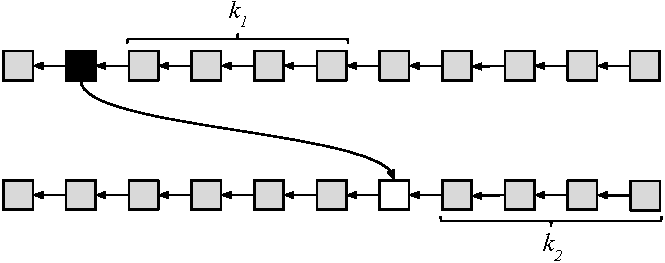
\includegraphics[width=0.7 \columnwidth,keepaspectratio]{figures/events.pdf}
    \label{fig.events}
\end{figure}

The operation of event reaction is shown in Figure~\ref{fig.events}. The process
is as follows. First, an event is fired in the source blockchain, shown at the
top. This could be any event that can be emitted using Ethereum's \textsc{emit}
command. This event firing is caused by a certain transaction which is included
at a certain block, indicated in black at the top. This block is the buried
under $k_1$ subsequent blocks within the source blockchain, where the $k_1$
parameter is a security parameter of the scheme depending on the specific
parameters of the source blockchain ~\cite{EC:GarKiaLeo15}. As soon as this
confirmation occurs, the event can be reacted to in the target blockchain, shown
at the bottom. This reaction occurs in a transaction which is included in a
block within the target blockchain, illustrated in white. As is usual even in
local blockchains, the block needs to be confirmed by waiting for $k_2$ blocks
to be mined on top of it. It is possible that $k_1 \neq k_2$ because of
different guarantees of different networks such as a difference in block
generation time or network synchronicity.

Using this basic functionality of event information exchange between
blockchains, we can construct two-way pegged sidechains. In such a construction,
an asset that exists on one blockchain, either as a \emph{native asset}, such as
ether in Ethereum, or as a \emph{token asset}, such as ICO or ERC20 tokens in
Ethereum, will gain the ability to be \emph{moved} to a different blockchain,
for example Ethereum Classic. We will use the example of moving ether from the
Ethereum blockchain and into the Ethereum Classic blockchain. Such an action is
different from \emph{exchanging} ether (ETH), the native token of the Ethereum
blockchain, with ether classic (ETC), the native token of the Ethereum Classic
blockchain. Instead, the asset retains its nature in that it maintains its price
and its ability to be used for the same purposes, while being governed by the
rules of the new blockchain, such as improved speed, limited fees, or better
features. Furthermore, no counterparty is required to exchange the asset; it is
something a party can do on its own.

Our constructions are fully decentralized and not require any sort of
federation.
